\documentclass[french,a4paper,12pt]{article} 
\usepackage[utf8]{inputenc}
\usepackage[T1]{fontenc}
\usepackage[a4paper,left=2cm,right=2cm,top=2cm,bottom=2cm]{geometry}
\usepackage{mathtools}
\usepackage[french]{babel}
\usepackage{perpage}
\usepackage{libertine}
\usepackage{blindtext}
\usepackage{babel}
\usepackage[pdftex]{graphicx}
\usepackage[rightcaption]{sidecap}
\usepackage{lmodern}
\usepackage{url}
\setlength{\parindent}{0cm}
\setlength{\parskip}{1ex plus 0.5ex minus 0.2ex}
\newcommand{\hsp}{\hspace{20pt}}
\newcommand{\HRule}{\rule{\linewidth}{0.5mm}}
\selectlanguage{french}
\title{Le Boosting en Machine Learning} % le titre de l'article
\author{Metango Kenfack Cathy Judith} 
\usepackage{caption,subcaption}
\tracinglostchars=2
\usepackage{iftex}
\pagestyle{plain}
\usepackage[authoryear]{natbib}
\ifTUTeX
  \usepackage{fontspec}
\else
  \usepackage[T1]{fontenc}
  \usepackage[utf8]{inputenc} % The default since 2018
  \DeclareUnicodeCharacter{200B}{{\hskip 0pt}}
\fi
\usepackage[]{tocbibind}
 \DeclareUnicodeCharacter{202F}{\,}

\begin{document}
\begin{titlepage}
  \begin{sffamily}
  \begin{center}
     
\includegraphics[scale=0.25]{logoulb.JPG}~\\[1.5cm]

    \textsc{\bfseries \LARGE Université Libre de Bruxelles }\\[0.5cm]
    \textsc{\Large Faculté de Lettres, Traduction et Communication}\\[6cm]

    % Title
    \HRule \\[0.4cm]
    { \huge \bfseries Le Boosting en Machine Learning\\[0.4cm] }

    \HRule \\[4cm]
    % Author and supervisor
    \begin{minipage}{0.4\textwidth}
      \begin{flushleft} \large
        Metango Kenfack Cathy \\

        
      \end{flushleft}
    \end{minipage}
    \begin{minipage}{0.4\textwidth}
      \begin{flushright} \large
        \emph{Travail réalisé sous la direction de DE VALERIOLA Sébastien dans le cadre du cours d'Architecture des Systèmes d'information (M-STIC-B540)} 
      \end{flushright}
    \end{minipage} \\ [2cm]

    \vfill

    % Bottom of the page
    {\large {} Année académique 2022-2023}

  \end{center}
  \end{sffamily}
\end{titlepage}


 %%fin de la parge de garde 
 \begin{center}
 \tableofcontents
 \end{center}
\newpage



\section{INTRODUCTION}
\quad Le thème soumis a notre étude est celui du Boosting en machine Learning. L’apprentissage automatique est une discipline qui permet d donner à un ordinateur la capacité d’apprendre à partir des données pour résoudre une tache qui implique généralement les prédictions. Il s’agit d’un sous-domaine de l'intelligence artificielle, qui est définie au sens large comme la capacité d'une machine à imiter le comportement humain intelligent. Les systèmes d'intelligence artificielle sont utilisés pour exécuter des tâches complexes d'une manière similaire à la façon dont les humains résolvent les problèmes. Apprentissage automatique utilisent pour ce fait des méthodes pour apprendre des informations à partir des données sans modèle de référencé prédéterminé. Il existe de ce faites plusieurs méthodes de machine Learning parmi lesquelles l’algorithme de boosting. Le boosting est un algorithme de machine Learning permettant de réduire les erreurs dans l’analyse prédictive des données. C’est une méthode d’ensemble Learning c’est a dire elle crée un modèle fort a partir d’un certain nombre de modèles faibles cela en demandant a chaque model de corriger les erreurs de son prédécesseur : les faiblesses des uns sont compensées par les forces des autres. L étude de ce projet porte sur cette notion qu’est le BOOSTING. Pour mener a bien cette étude nous nous aborderons plusieurs points. Définir boosting et machine Learning, donner l’importance du boosting, présenter le principe et fonctionnement du ce dernier , expliquer un exemple d’algorithme du boosting avec un exemple d’application . 




\newpage
\section{Machine Learning}
\subsection{Définition}
\quad Vous ami a du mal à faire une différence entre le citron et la mandarine avec suffisamment de précision pour la reconnaitre dans un supermarché. Mais si vous lui montrez quelques-unes de ses photos, il repérera immédiatement les traits révélateurs dont il a besoin. Comme on dit, une image, un exemple, vaut mille mots supposons ici que votre ami c’est votre machine et qu’on aimerait apprendre à la machine à distinguer les citrons des mandarines. Plutôt que de coder une machine avec des images représentatifs des citrons et mandarines, nous pouvons plutôt programmer la machine pour apprendre à les distinguer grâce à une expérience répétée avec les citrons et les mandarines réelles. C’est ça le machine Learning donner la capacite à un ordinateur d’apprendre à partir des données.

\quad Incapables de définir certains objets ou concepts avec suffisamment de précision, nous voulons les transmettre à la machine au moyen d'exemples. Pour que cela fonctionne, cependant, l'ordinateur doit avoir la capacite de convertir les exemples fournis par l’humain pendant l’apprentissage en connaissances. Une fois que cette phase d’apprentissage est faite, on peut faire des prédictions c’est à dire produire une réponse correcte sur les données similaires mais sur lesquelles le programme n’a pas été entrainée.   D'où l’intérêt pour les algorithmes d’apprentissage automatique, le sujet de ce manuel.

\quad Le machine Learning est donc une branche évolutive des algorithmes ayant pour but d’imiter la capacite humaine. Elle s’appuie sur notions de déférentes disciplines telles que informatique, l’intelligence artificielle, les probabilités et statistiques, la psychologie,  Elle a montré son importance et elle est applique dans plusieurs domaines varie de la vie tel qu’en finance pour la prédiction du chiffre d’affaires, la détection de fraude, en transport pour la prédiction du nombre d’accident en politique pour la prédiction de résultat, en biologie, en divertissement, en marketing , en médecine , en biomédecine, en physique médicale et bien encore.



\quad Nous allons donc pour notre travail montrer comment le machine Learning grâce aux algorithmes pour faire des prédictions. Plusieurs algorithmes apprentissage automatique existe, mais dans notre cas nous parlerons de l’algorithme de Boosting.

\subsection{ fonctionnements du machine Learning : apprendre à partir des données }

\quad Les machines pour qu’elles apprennent ont besoin des données (images, sons, textes, vidéos, prix d’une maison). Ce processus en apprentissage automatique est appelé expérience. Après avoir donné ces donnes à la machine on doit par suite préciser la tache quelle doit réaliser (catégoriser les images, prédire le prix d’une maison, prédire le chiffre d’affaires). En fonction de la tache quelle a appris nous devons à la fin évaluer son apprentissage pour mesurer sa performance. Il existe donc pour ce fait des algorithmes d’apprentissages. Le machine Learning regroupe trois grandes familles d’algorithme d’apprentissage : apprentissage supervisé, apprentissage non supervisé et apprentissage semi supervisé. En fonction du type d’apprentissage nous avons plusieurs algorithmes, mais comme énoncé plus haut nous parlerons d’algorithme de boosting qui est un algorithme d’apprentissage supervisé. 

\section{Algorithme de Boosting}
\quad Dans cette section, nous donnerons les raisons pour lesquelles le boosting est utilise, ensuite nous allons la  defini , ensuite presenter son fonctionnement et enfin illustrer les differents types algorithme boosting.

 \subsection{Enjeux : Pourquoi le boosting est til utilise}

\quad Avec le development de la technologies , le progrs dans les divers domaines tells que le marketing , la sante , les finance , etc…, il est necessaires de développer des techniques d'apprentissage automatique plus complexes et plus avancees. 

\quad Le boosting est une technique qui peut etre utilisee pour resoudre des problemes complexes , bases sur des donnees et le monde reel.
Supposons qu'on veux   créer un modèle pour un ensemble de données d'images contenant des images de chats et de chiens et que nous voulons classer ces images en deux classes différentes. Nous allons pour cela  commencez par identifier les images en fonction de certaines règles, telles que les éléments suivants : 
La photo a des oreilles pointues : chat
L'image est un œil en forme de chat : chat
L'image a de grands membres : chien
L'image a des griffes aiguisees : chat
L'image a une structure de bouche plus large : chien

\quad En effet , les prédictions de chacun de ces apprenants faibles peuvent être combinées avec une règle de majorité ou une moyenne pondérée pour rendre les prédictions plus précises. Cela en fait de solides modèles d'apprentissage.
Dans lexemple ci dessus, nous avons defini 5 classificateurs faibles et  la majorite de ces regles (3 classificateurs sur 5 predisent limage comme un chat) nous donne la prediction que l’image est un chat. On conclus que notre sortie est un chat. Ceci nous amene a nous pose la question ci après.

\subsection{Définition}

 \quad Le boosting est une technique d’ensemble general qui cree un apprenant fort a partir d’un certains nombre d’apprenant faibles. Cela se fait en construisant un modele à partir des donnees d’apprentissage puis en creant un deuxieme modele qui tente de corriger les erreurs du model precedent. 

 \begin{center}
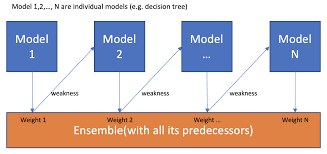
\includegraphics[scale=1]{boosting definition.png}
\begin{figure}[h]
\caption{Présentation de la technique du Boosting}
\end{figure}
\end{center}
\subsection{ Ensemble learning}

\quad En regroupant un ensemble de modeles , on obtiens ume meilleurs performance que lorsqu’on utilise nos modèles chacun de leur cote. Cette methode est base sur le concept The wisdom of the crowd qui est un phenomene lie a la loi des grands nombres qui fait qune foule d’individus a souvent plus raison qu’un expert tout seul  a condition que la foule soit grande et diversifieée (les modèles doivent etres différent, construit sur des données différents ou avec des algorithms d’apprentissage différents)et compétente. En apprentissage automatique on peu  utiliser ce concept pour creer un ensemble de modeles qui surpassent les performances des meilleures modeles de machine d’apprentissage au monde. Pour cela on distingue 3 grandes techniques qui sont : le Bagging , le Boosting et le Stacking.  

\textbf{le Boosting} 
\quad Ici, les apprenants faibles sont générés séquentiellement  , en demandant à chaque modèle de corriger les erreurs de son predécesseur, on n’a donc toujours un nouvel algorithme formé sur les mauvaises predictions faites précédemment. En attribuant des poids plus élevés aux échantillons précédemment mal classés, les performances du modèle sont améliorées. Un exemple de boosting est l'algorithme AdaBoost.

\textbf{Le Bagging} 
\quad les apprenants faibles sont produits parallèlement. Ici , les données sont echantillonnées (le boosstrapping) et on obtenir un ensemble de models diversivié en entrenant sur une portion aleatoire de données chaque modèle. La prediction finale est la moyenne des predictions de chaque modèles qui ont été prealablement obtenus. 

\textbf{Le Stacking}
\quad cette technique consiste à entrainer plusieurs modèles différents avec les meme données puis utilizer les resultats des différents modèles  sur un modèle final qui donne la prediction finale. Elle permet entrainer un modèle d ‘apprentissage à reconnaitre qui a tort et qui a raison dans un ensembles de modèles, ceci améliore encore plus la performance générale. 


 \begin{center}
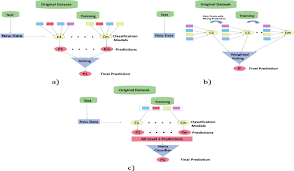
\includegraphics[scale=1]{Techniques ensembles learning.png}
\begin{figure}[h]
\caption{: ensemble Learning Methods (a = Bagging, b = Boosting, c = Stacking)}
\end{figure}
\end{center}

\subsection{Fonctionnement du boosting}
\quad Le principe de base de algorithmes de boosting est de générer plusieurs apprenants faibles et de combiner leurs prédictions pour former un apprenant fort. Ces apprenants faibles sont générés en appliquant des algorithmes d'apprentissage automatique de base à différentes distributions de l'ensemble de données. Ces algorithmes génèrent des règles faibles à chaque itération. Après quelques itérations, les apprenants faibles sont combinés en apprenants forts qui prédisent des résultats plus précis.



\textbf{étape 1}

 \quad L'algorithme de base lit les données et attribue des poids égaux à chaque observation d'échantillon de données. Puis algorithme de base faire des predictions pour chacun de ces échantillons.
 
 \textbf{étape 2}
 \quad L’algorithme identifie les prédictions incorrectes faites par les apprenants de base. À l'itération suivante, ces prédictions erronées sont attribuées à l'apprenant de base suivant avec des poids plus élevés pour ces prédictions erronées.

 
 \textbf{étape 3}
\quad on répète l'étape 2 jusqu'à ce que l'algorithme puisse apprendre correctement.
Par conséquent, l'objectif principal du boosting est de se concentrer davantage sur les prédictions erronées.

\quad Maintenant que nous connaissons comment fonctionne l’algorithme de boosting, intéressons-nous maintenant aux différents types de algorithme de boosting. Mais avant nous présenterons des Forces  et Faiblesses de celui ci.


\begin{center}
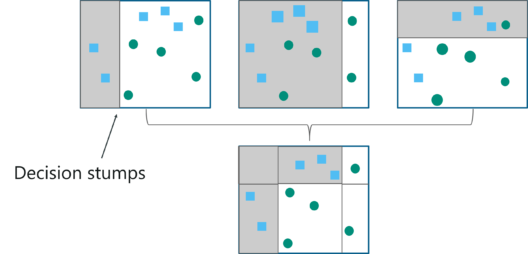
\includegraphics[scale=1]{fonctionnement boosting.png}
\begin{figure}[h]
\caption{: fonctionnement de Algorithme Boosting}
\end{figure}
\end{center}


























\newpage
\section{Conclusion}






\newpage
\begin{center}
\listoffigures
\end{center}

\newpage

\begin{center}
\bibliography{bibio}
\bibliographystyle{unsrtnat}
\end{center}

\end{document}
